% !TeX spellcheck = en_US
\documentclass[12pt,a4paper,titlepage]{article}
\usepackage[utf8]{inputenc}
\usepackage[T1]{fontenc}
\usepackage{amsmath}
\usepackage{amsfonts}
\usepackage{amssymb}
\usepackage{makeidx}
\usepackage{svg}
\usepackage{graphicx}
\usepackage[left=2.00cm, right=2.00cm, top=2.00cm, bottom=2.00cm]{geometry}
\usepackage{tikz}
\usepackage{tikz-uml}
\usepackage{wallpaper}
\linespread{1.3}
\usetikzlibrary{patterns}%for tikz https://tex.stackexchange.com/questions/54464/hatch-a-rectangle-in-tikz
\usetikzlibrary{svg.path}
%sources
\usepackage[backend=bibtex,style=alphabetic]{biblatex}
\bibliography{Thesis}

%Captions for figures in minipage
\usepackage{caption}

%Makes index browsable in pdf viewers and shows index in sidebar
\usepackage[hidelinks]{hyperref}
%Ensures that \ref works with paragraphfs as intended
\setcounter{secnumdepth}{6}

%For svg images in subdirectory
\graphicspath{{res/images/}}

\begin{document}	
	\begin{titlepage}
		\ThisCenterWallPaper{1}{"./res/images/titleImageReworked.jpeg"}
		\null
		\newpage
	\end{titlepage}
	
	\pagenumbering{roman}
	\tableofcontents
	\listoffigures
	\clearpage
	\pagenumbering{arabic}
	\let\oldref\ref
	\renewcommand{\ref}[1]{\oldref{#1} (page~\pageref{#1})}
	
	\section{Abstract}
	This paper describes the coding of a program in Java and OpenCL capable of calculating a few selected fractals and casts light on the core aspects I have implemented, such as how the data is calculated and stored. The paper will first explain what a fractal is, albeit only briefly since they do not have to be discussed in depth for my use case. The next section \ref{sec:fractals} shortly describes the functionalities and the structure of my program, breaking it down into logical components depending what they are responsible for. The last section is dedicated to bugs, known issues and their workarounds, limitations and possible ways of improving of my program, followed by a reflection on my work.
	\section{What are Fractals?}\label{sec:fractals}
	Mathematicians used to rely exclusively on classical algebra to describe as well as research sets and functions. As classical algebra is only able to describe regular sets and functions, any irregular set could not by described and ended up being labeled as pathological, irrelevant and not being paid any further attention. This decision however was found to be a fallacy, as irregular functions and sets provide a better representation of natural phenomenons and structures (for example coast lines, cloud borders, turbulence in fluids, snow flakes (see figure \ref{fig:snowflake})) than normal shapes described by classical geometry. These irregular sets and functions are now known as fractals. 
	While they were first conceptualized by Felix Hausdorff in 1918, it was only in the 1970s, after the advent of computers with their impressive computational power, that the exploration of fractals became much easier. The term fractal (from Latin \emph{fragmented, broken}) ) was coined in 1975 by mathematician Benoît B. Mandelbrot. Mandelbrot used fractals as a tool to examine the stock market, but they have proved to be useful in various fields like physical chemistry, fluid mechanics and physiology \cite{FalconerKennethJ1993FG:m, britannica}.
	\subsection{The Sierpiński Triangle}
	The properties of fractals will be illustrated utilizing with the aid of the Sierpiński triangle (figure \ref{fig:sierpinski_triangle}). The structure, while seeming complex at first glance, reveals a rather simple creation process. As illustrated in figure \ref{fig:sierpinski_triangle_build} the construction starts with a filled triangle which is split into three smaller triangles by cutting out an triangular upside-down hole. The resulting triangles are once again cut out, creating more triangles. This process is repeated \emph{ad infinitum} on any newly created triangles. \\
	The first notable property is the perfect self similarity. An infinite amount of scaled down copies of the fractal can be found in the original structure. This property is also found in other fractals, including the Mandelbrot or Julia set, although the copies often only resemble the original approximately. Some fractals display a statistical self similarity, meaning that the copies statistically show the same properties at many scales.\\
	The next property is indirectly a predecessor of the aforementioned self similarity. Fractals have to contain a certain microstructure. The Sierpiński triangle can be magnified infinitely without ever showing a final structure which is not fractured itself. Additionally, the local geometry cannot be described by classical Euclidean (meaning shapes like circles, lines, spheres, cuboids and such) geometry; the structure is by far not adequately regular.\\
	Contrary to its appearance, the definition of the Sierpiński triangle is thus quite simple. Furthermore, it is a recursive. Both these properties are often also characteristic of other fractals.\\
	Although it lies outside the scope of this paper, the Hausdorff dimension is also worth mentioning. Broadly speaking, the Hausdorff dimension is a real number (as opposed to the topological dimensions, which are always integers) which describes how much space a set fills up and it is usually greater than its topological dimension \cite[Einleitung]{FalconerKennethJ1993FG:m}.
	
	\begin{figure}
		\caption{Sierpiński triangle \cite{sierpinski_image}}
		\label{fig:sierpinski_triangle}
		\centering
		\includegraphics[width=0.5\textwidth]{"res/images/1000px-Sierpinski_triangle.svg.png"}
	\end{figure}
	\begin{figure}
		\caption{Each branch of the snowflake creates new smaller branches \cite{wikipedia_snowflake}}
		\label{fig:snowflake}
		\centering
		\includegraphics[width=0.5\textwidth]{"res/images/bentley_snowflake.jpg"}
	\end{figure}
	\begin{figure}
		\caption{Creation of the Sierpinski triangle}
		\label{fig:sierpinski_triangle_build}
		\centering
		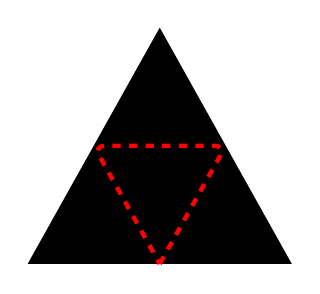
\begin{tikzpicture}[scale=3]
		\fill[black] (0,0) -- (1.118,0) -- (1.118/2, 1);
		
		\draw[rounded corners, dashed, red, ultra thick] (1.118/2, 0) -- (1.118/4*3,.5) -- (1.118/4, .5) -- (1.118/2, 0);
		\end{tikzpicture}
		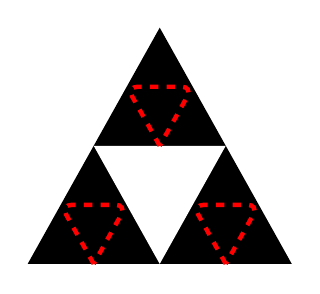
\begin{tikzpicture}[scale=3]
		\fill[black] (0,0) -- (1.118033989,0) -- (1.118033989/2, 1);
		\fill[white] (1.118/2, 0) -- (1.118/4*3,.5) -- (1.118/4, .5);
		
		\draw[rounded corners, dashed, red, ultra thick] (1.118/4*3, 0) -- (1.118/8*5,.25) -- (1.118/8*7, .25) -- (1.118/4*3, 0);
		\draw[rounded corners, dashed, red, ultra thick] (1.118/4, 0) -- (1.118/8,.25) -- (1.118/8*3, .25) -- (1.118/4, 0);
		\draw[rounded corners, dashed, red, ultra thick] (1.118/2, .5) -- (1.118/8*3,.75) -- (1.118/8*5, .75) -- (1.118/2, .5);
		\end{tikzpicture}
		
\begin{tikzpicture}[scale=3]
		\fill[black] (0,0) -- (1.118033989,0) -- (1.118033989/2, 1);
		
		\fill[white] (1.118/2, 0) -- (1.118/4*3,.5) -- (1.118/4, .5);
		
		\fill[white] (1.118/4*3, 0) -- (1.118/8*5,.25) -- (1.118/8*7, .25);
		\fill[white] (1.118/4, 0) -- (1.118/8,.25) -- (1.118/8*3, .25);
		\fill[white] (1.118/2, .5) -- (1.118/8*3,.75) -- (1.118/8*5, .75);
		\end{tikzpicture}
	\end{figure}
	
	\subsection{The Mandelbrot Set}
	Although most of my senior thesis revolves around computer science the necessity arises to explain the fractal crucial in my work. The Mandelbrot set was named after Benoît B. Mandelbrot, and is the first one to be called a fractal. In terms of properties, it is related to the Julia set, which is also not a part of my work, although my program has the ability to display it. The Mandelbrot set \(\mathbb{M}\) is an, unlike the previously mentioned geometric Sierpiński triangle, the Mandelbrot set \(\mathbb{M}\) is an algebraic fractal in the complex plane \(\mathbb{C}\). There are multiple definitions for the set, but the most relevant for my work is as follows:
	\begin{align*}
			f_{c}(z)&=z^2 + c\\
			f_{c}^{n} &= f_{c} \circ f_{c} \dots \circ f_{c}\\
			\mathbb{M} &= \{c \in \mathbb{C}: f_{c}^{n}(0)\not\to\infty \text{ for } n \to \infty\}
	\end{align*}
	Each point \(c \in \mathbb{C}\) has a corresponding function \(f_c(z)=z^2 +c\). Now let \(z_0=0\), \(z_1 = f_c(z_0)\), \(z_2 = f_c(f_c(z_0))\), or more generally \(z_n = f_c(f_c(\dots f_c(0)))= f_c^n(0)\). The example below may be more easily understood with the recursive definition \(z_{n+1}=z_n^2+c\). \(z_k\) is called the \(k\)th iteration of a point. If \(|z_n|\) grows to infinity for \(n \to \infty\), \(c\) is not part of the set. On the other hand, if \(|z_n|\) tends to a finite number, \(c\) is part of the set.\\
	Table \ref{fig:iterations_mandelbrot} shows the first ten iterations of two examples. It is trivial that \(z_1=c\), since \(z_0 = 0\). While \(z_n\) diverges quickly for \(c=0.9 - 0.2i\), it remains small and does not tend to infinity for \(c=0.3+0.2i\). For any other \(c\) it may take hundreds of thousand of iterations to diverge. Whilst no proof will be provided, since it lies outside the scope of this paper, it can be shown that \(\lim_{n\to\infty}z_{n} = \infty\) if \(|z_{k}| > 2\) for any \(k\), meaning that further iterations are not necessary to determine that a point is not part of the set. Theoretically, a point has to go through an infinite amount of iterations to prove that it is part of the set and does not diverge. To complete this obviously unaccomplishable task, programs usually only calculate a limited amount of iterations and give up as soon as that maximum is reached. Raising the limit creates more detail in the fractal at the cost of calculation time, but this is only necessary when magnifying the set \cite[Chapter 14.2]{FalconerKennethJ1993FG:m}.
	\begin{figure}
		\centering
		\caption{Iterations of different \(c\)}
		\label{fig:iterations_mandelbrot}
		\begin{minipage}{.45\textwidth}
			\centering
			\begin{tabular}{c|l}
				\multicolumn{2}{c}{\(c=0.3+0.2i\)} \\ \hline
				\(z_1\)& \(0.3\, -0.2 i\)\\ \hline
				\(z_2\)& \(0.35\, -0.32 i\)\\ \hline
				\(z_3\)& \(0.3201\, -0.424 i\)\\ \hline
				\(z_4\)& \(0.222688\, -0.471445 i\)\\ \hline
				\(z_5\)& \(0.12733\, -0.40997 i\)\\ \hline
				\(z_6\)& \(0.148137\, -0.304403 i\)\\ \hline
				\(z_7\)& \(0.229284\, -0.290187 i\)\\ \hline
				\(z_8\)& \(0.268363\, -0.33307 i \)\\ \hline
			\end{tabular}
		\end{minipage}
		\begin{minipage}{.45\textwidth}
			\centering
			\begin{tabular}{c|l}
				\multicolumn{2}{c}{\(c=0.9-0.2i\)} \\ \hline
				\(z_1\)& \(0.9\, + 0.2 i\)            \\ \hline
				\(z_2\)& \(1.67\, +0.56 i\)            \\ \hline
				\(z_3\)& \(3.3753\, +2.0704 i\)           \\ \hline
				\(z_4\)& \(8.00609\, +14.1764 i\)            \\ \hline
				\(z_5\)& \(-135.974+227.196 i\)            \\ \hline
				\(z_6\)& \(-33128.1-61785.2 i\) \\ \hline
				\(z_7\)& \(-2.71994\times 10^9+4.09366\times 10^9 i\)           \\ \hline
				\(z_8\)& \(-9.35996\times 10^{18}-2.2269\times 10^{19} i\) \\ \hline
			\end{tabular}
		\end{minipage}
	\end{figure}
	\begin{figure}
		\caption{The Mandelbrot set}
		\label{fig:mandelbrot}
		\centering
		\includegraphics[width=0.5\textwidth]{"res/images/mandelbrot.png"}
	\end{figure}
	\section{The Program}
	This section represents the core of my paper. It starts by listing the capabilities of my program without giving technical details to the underlying model, which in turn is described as next. Lastly, the implementation is discussed.
	\subsection{Program Functionalities}
	My program is able to calculate and render fractals. Before starting the calculation engine, parameters of the calculation can be set, for example the maximal amount of iterations a point can go through before assuming that it is part of the Mandelbrot set. Once the render engine has been started, the user can move around and zoom into the fractal. Should an interesting spot be identified, the user can export the location as an image and save it to the disk. It is also possible to create an animation and export it as a video. The export dialog offers the option to change the resolution. The raw calculation data may also be saved to, or loaded from, the disk.\\
	Users familiar with OpenCL can also modify the calculation and render kernel in order to change the fractal and coloring function. Depending on how many iterations are requested by the user massive computing power is needed. Should the local power not suffice to achieve the result in useful time, it is possible to harness the computing power of multiple computers by connecting them to each other. One machine then acts as the ``master'' and coordinates all the other machines (``slaves''), while they in turn calculate the fractal.	
	\subsection{Structure}
	Programs are usually programmed in a divide-and-conquer manner. Instead of implementing the project as a whole, it is split in smaller non autonomous sub modules. This has several advantages. Because the code is grouped in smaller modules, the project is easier to maintain over time as specific pieces of code can be found easier when the need to edit them arises. Also, other coders will understand the code better if it is structured practically.\\
	Another perk is the ease of debugging. The modules are like links tied together in a chain. When the program has to do something, the first link receives an order to do what it was programmed to and passes an interim result to the next link, which does another calculation composing a new interim result. This process is repeated until the end of the chain is reached where the final result is created. A single faulty link out of thousands will likely screw up the entire procedure. The search for the culprit, alias debugging, is much easier when the code is not written in a single big block, because the interim results can be inspected, betraying any faulty links. It is also possible to test a single modules (unit testing) instead of the whole program.\\
	Figure \ref{fig:program_structure} shows how the code is grouped and structured in smaller components, as well as how they interact with each other. The harshest division is between the core, which encapsulates the logic to calculate, store and render data, and the GUI (graphical user interface) which offers a window for the user to interact with. This is because a programmer may wish to use the calculation capabilities in his own program and no GUI is needed. This way the GUI can be easily omitted.\\
	The next section will only briefly describe how the single modules work, starting with the core components and then moving on to the less complex GUI. An in-depth discussion will follow in section \ref{sec:implementation}.
	\begin{figure}
		\centering
		\caption{Program structure}
		\label{fig:program_structure}
		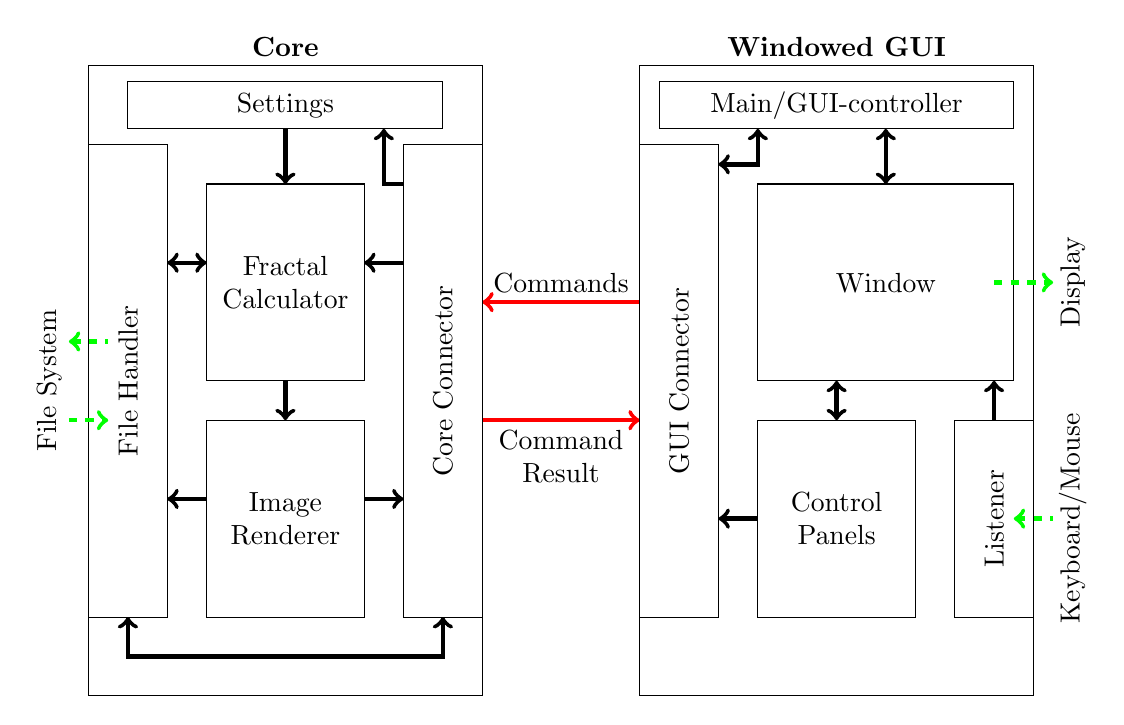
\begin{tikzpicture}
		%Front/Backend-connection
		\draw[red, ultra thick, <-] (5,5) -- (7,5);
		\node[above, align=center] at (6,5) {Commands};
		
		\draw[red, ultra thick, ->] (5,3.5) -- (7,3.5);
		\node[below, align=center] at (6,3.5) {Command\\Result};
		
		%Backend
		\draw (0,0) rectangle (5,8);
		\node[above] at (2.5, 8) {\textbf{Core}};
		
		%Interface
		\draw (4,1) rectangle (5, 7);
		\node[rotate = 90] at(4.5, 4) {Core Connector};
		
		%Settings
		\draw (.5,7.2) rectangle (4.5, 7.8);
		\node at (2.5, 7.5) {Settings};
		
		%Fractal calculator
		\draw (1.5,4) rectangle (3.5, 6.5);
		\node[align=center] at (2.5, 5.25) {Fractal\\Calculator};
		
		%Image render
		\draw (1.5,1) rectangle (3.5, 3.5);
		\node[align=center] at (2.5, 2.25) {Image\\Renderer};
		
		%File handling
		\draw (0,1) rectangle (1, 7);
		\node[rotate = 90] at(.5, 4) {File Handler};
		
		%Arrows
		%Settings-Frac
		\draw[ultra thick, ->] (2.5, 7.2) -- (2.5, 6.5);
		%Int-Frac
		\draw[ultra thick, <-] (3.5, 5.5) -- (4, 5.5);
		%Frac-Image
		\draw[ultra thick, ->]  (2.5, 4) -- (2.5, 3.5);
		%Img-Int
		\draw[ultra thick, ->]  (3.5, 2.5) -- (4, 2.5);
		%Frac-File
		\draw[ultra thick, <->] (1.5, 5.5) -- (1, 5.5);
		%Image-File
		\draw[ultra thick, ->] (1.5, 2.5) -- (1, 2.5);
		%Settings-Int
		\draw[ultra thick, ->] (4, 6.5) -- (3.75, 6.5) -- (3.75, 7.2); 
		%Int-File
		\draw[ultra thick, <->] (4.5, 1) -- (4.5,.5) -- (.5,.5) -- (.5, 1);
		
		%File system
		\draw[green, ultra thick, dashed, ->] (-.25, 3.5) -- (.25, 3.5);
		\draw[green, ultra thick, dashed, <-] (-.25, 4.5) -- (.25, 4.5);
		\node[rotate = 90] at (-.5, 4) {File System};
		
		%Frontend
		\draw (7,0) rectangle (12,8);
		\node[above] at (9.5, 8) {\textbf{Windowed GUI}};
		
		%Interface
		\draw (7,1) rectangle (8, 7);
		\node[rotate = 90] at(7.5, 4) {GUI Connector};
		
		%Main
		\draw (7.25,7.2) rectangle (11.75, 7.8);
		\node at (9.5, 7.5) {Main/GUI-controller};
		
		%Window
		\draw (8.5,4) rectangle (11.75, 6.5);
		\node[align=center] at (10.125, 5.25) {Window};
		
		%Control Panels
		\draw (8.5,1) rectangle (10.5, 3.5);
		\node[align=center] at (9.5, 2.25) {Control\\Panels};
		
		%Listener
		\draw (11,1) rectangle (12, 3.5);
		\node[rotate = 90] at(11.5, 2.25) {Listener};
		
		%Arrows
		%Main-Win
		\draw[ultra thick, <->] (10.125 ,7.2) -- (10.125, 6.5);
		%List-Win
		\draw[ultra thick, ->] (11.5, 3.5) -- (11.5,4);
		%Ctr-Win
		\draw[ultra thick, <->] (9.5, 3.5) -- (9.5, 4);
		%Main-Interface
		\draw[ultra thick, <->] (8, 6.75) -- (8.5, 6.75) -- (8.5, 7.2);
		
		%Ctr-Interface
		\draw[ultra thick, <-] (8, 2.25) -- (8.5, 2.25);
		
		%Keyboard/Mouse
		\draw[green, ultra thick, dashed, ->] (11.5, 5.25) -- (12.25,5.25);
		\node[rotate = 90] at (12.5, 5.25) {Display};
		
		\draw[green, ultra thick, dashed, <-] (11.75, 2.25) -- (12.25, 2.25);
		\node[rotate = 90] at (12.5, 2.25) {Keyboard/Mouse};
		\end{tikzpicture}
	\end{figure}
	
	\subsubsection{Core}
	The core consists of multiple components or units, which are tightly bound together. Each of them is responsible for a certain task and should not do anything else. The modules are capable of communicating to the connector, and in some cases each other, but are isolated from the ``outside'', with the exception of the connector and file handler. These two interchange data with either the UI or the underlying file system.
	\paragraph{Settings}
	The settings are configurations used either directly during computation or as parameters for the program itself. Variables used during the computation could be for example the maximal number of iterations allowed  or the color function used when rendering the data. The settings can only be changed before the actual fractal calculator is started.
	\paragraph{Database}
	The data model is the one of the most complex parts of my project, as the data has to have low access times to lots of data. To achieve this, the data is logically split multiple times. The topmost containers are called levels and sort the data by precision (more to that in section \ref{sec:implementation}). They do not contain the data directly but instead are made up by clusters, which store small chunks of data sorted by location. The size of these chunks is determined by the settings.
	\paragraph{Fractal Calculator}
	The calculator determines if points are part of the set, and if not how many iterations it takes to be sure that the point is not in the set. It contains the logic to harness the power graphic cards provide using OpenCL and can even connect to other computers to use their computing power as well.
	\paragraph{Renderer}
	The renderer converts raw data to an image. The amount of iterations a point has gone through before it escaped the set is mapped to a specific color depending on the color function defined.
	\paragraph{Connector}
	The connector conduces all the components and provides the API to control the core, meaning that the GUI can issue commands only through the connector. This adds an extra level of abstraction, as the GUI does not have to worry about how the core calculates data and only has to request an image. 
	\subsubsection{GUI}
	The GUI is the face my program has when utilized. Although most of my efforts have gone towards developing the core, a stable GUI still had to be developed. The application consists of a simple main window and an occasional popup when user input such selecting a file is required.
	\paragraph{Login}
	Upon starting the application, a login screen is displayed. The user can adjust the settings by opening the settings dialog and edit the calculation and render kernel if he has the knowledge to. It is also possible to start the application as a slave.\\
	When the start button is pressed, the user can select which computer parts are used to render the fractal. Usually, only installed GPUs will show up as an option, but machines with OpenCL support on the CPU will also show a CPU. If the program accepts external slaves they will also show up as options. After confirming the selection the program changes to the master view. If the slave option was selected, the program attempts to connect to the specified master and shows the slave view, which is empty.
	\paragraph{Master View}
	The master view consists of the fractal in the middle and a menu bar on top containing entries to export images or videos and save calculated data. By left clicking and dragging the mouse the user is able to move around. Dragging using the right mouse button selects an area which will be magnified. It is also possible to zoom using the mouse wheel. Alternatively, the viewport can also changed via the menu bar.
	\subsection{Core Implementation}\label{sec:implementation}
	This section discusses the functionalities in greater depth, although without going into the Java specific implementations, i.e. no classes or class methods will be mentioned.\\
	Whilst this kind of in depth documentation could be written too about the GUI I have not written one, since the GUI is neither as complex nor interesting as the core. Not only for this reason have I also invested lots of more time in the core than the GUI.
	\subsubsection{Dataset}
	The connector passes the data generated from the calculator to the dataset where it is stored. The data consists of points (or mathematically speaking complex numbers) which each have a value corresponding to the amount of iterations the program has applied to a point. To facilitate further use, the point and its value are from now on grouped in a structure called entry. Table \ref{fig:entries} shows three entries with values. The \(-1\) denotes that the point did not diverge and is thus in the Mandelbrot set.
	\begin{figure}
		\centering
		\caption{A table containing entries}
		\label{fig:entries}
		\begin{tabular}{c|c}
			Point        & Value \\ \hline
			\(0.3+0.3i\) & -1    \\ \hline
			\(0.4+0.2i\) & 31    \\ \hline
			\(0.4+0.5i\) & 7     \\
		\end{tabular}
	\end{figure}
	\paragraph{General Understanding}
	
%TODO does this help?
%	\begin{figure}
%		\caption{Schematic of the dataset}
%		\label{fig:dataset_schematic}
%		\centering
%		\def\svgwidth{\textwidth}
%		\input{res/images/dataset.pdf_tex}
%	\end{figure}

	This section gives an insight on how the data is sorted in the dataset without going into mathematical details, which will done in the following sections \ref{sec:clusters} and \ref{sec:levels}. Figure \ref{fig:dataset} illustrates the separation of points of the set (green) into clusters (red) and levels (blue). The topmost square shows the entire ``raw'' dataset and the three following squares each show a level with clusters.\\
	To understand the model further the purpose of the data has to be considered, which is generating images. Broadly speaking, every pixel represents a point in the dataset. Because all pixels have the same distance to their neighboring pixels all points needed have the same distance to their neighboring points. It is thus sensible to sort points by their distance to their neighbors. This makes it possible to quickly query the necessary points when an image is rendered instead of having to search the entire dataset. This is put to practice by the so called levels.\\
	Furthermore, the image often only shows a part of the area the dataset spans over, meaning that only the points in that part of the area are needed. The image creation process will thus mostly need a part a level's points. Since the points needed are also always close to each other, it makes sense to group the points by their location in small chunks, called clusters in my program. Their advantage is that they can be queried much faster than single values.\\	
	I take the limitations of this dataset model beforehand: It can only store points which are in the bounds of the dataset and lie on an invisible grid. The dataset requires that data added fits into the present structure. It might seem a bit baffling that it is only capable of storing certain points, but for the purpose needed this actually facilitates the image generation process because the data can be directly mapped to an image, see section \ref{sec:image_generation}.
	\begin{figure}
		\centering
		\caption{An exemplary dataset with \(L_0\) to \(L_2\)}
		\label{fig:dataset}
		\begin{minipage}{.4\textwidth}
			\centering
			\begin{tikzpicture}
			\node at (2,2) {\includegraphics[width=4cm, height=4cm]{res/images/mandelbrot.png}};
			\draw[thick, orange, ->] (-.3,2) -- (4.3,2) node[right]{\(Re\)};
			\draw[thick, orange, ->] (2,-.3) -- (2,4.3) node[right]{\(Im\)};
			\draw[ultra thick] (0,0) rectangle (4,4);
			\foreach \x in {0,...,15} {
				\foreach \y in {0,...,15}{
					\fill[green] (.25 * \x + .125, .25 * \y + .125) circle[radius=.05];
				}	
			}
			\draw[orange](1.9,3) -- (2.1,3) node[right] {\(i\)};
			\draw[orange](1.9,4) -- (2.1,4) node[right] {\(2i\)};
			\draw[orange](3,1.9) -- (3,2.1) node[above] {\(1\)};
			\draw[orange](4,1.9) -- (4,2.1) node[above] {\(2\)};
			\end{tikzpicture}
		\end{minipage}\\
		\begin{minipage}{.4\textwidth}
			\centering
			\begin{tikzpicture}
			\node at (2,2) {\includegraphics[width=4cm, height=4cm]{res/images/mandelbrot.png}};
			\draw[ultra thick, blue] (0,0) rectangle (4,4);
			\draw[step=2,red, dashed] (0,0) grid (4,4);
			\foreach \x in {0,...,3} {
				\foreach \y in {0,...,3}{
					\fill[green] (1 * \x + .5,1 * \y + .5) circle[radius=.05];
				}
			}
			\draw[red, |<->|] (0,-.2) -- (1,-.2) node[below, align = center] {\(c_{a,w}= 2\)\\\(c_{l,w}= 2\)} -- (2,-.2);
			\draw[blue, |<->|] (0,4.2) -- (2,4.2) node[above, align = center] {\(l_{a,w} = 4\)\\\(l_{l,w} = 2\)}-- (4,4.2);
			\draw[blue, |<->|] (4.2, 0) -- (4.2,2) node[right, align = center] {\(l_{a,h} = 4\)\\\(l_{l,h} = 2\)}-- (4.2,4);
			\node[right] at (3,-.8) {\(p(L_0)= \frac{2}{2} = 1\)};
			\node[blue] at (-1,2) {\(L_0\)};
			\end{tikzpicture}
		\end{minipage}
		\begin{minipage}{.4\textwidth}
			\centering
			\begin{tikzpicture}
			\node at (2,2) {\includegraphics[width=4cm, height=4cm]{res/images/mandelbrot.png}};
			\draw[ultra thick, blue] (0,0) rectangle (4,4);
			\draw[step=1,red, dashed] (0,0) grid (4,4);
			\foreach \x in {0,...,7} {
				\foreach \y in {0,...,7}{
					\fill[green] (.5 * \x + .25,.5 * \y + .25) circle[radius=.05];
				}
			}
			\draw[red, |<->|] (0,-.2) -- (.5,-.2) node[below, align = center] {\(c_{a,w}= 1\)\\\(c_{l,w}= 2\)} -- (1,-.2);
			\draw[blue, |<->|] (0,4.2) -- (2,4.2) node[above, align = center] {\(l_{a,w} = 4\)\\\(l_{l,w} = 4\)}-- (4,4.2);
			\draw[blue, |<->|] (4.2, 0) -- (4.2,2) node[right, align = center] {\(l_{a,h} = 4\)\\\(l_{l,h} = 4\)}-- (4.2,4);
			\draw[->, red] (2.5, -.2) node[below] {\(C_{2,0}=C_2\)}-- (2.5,.5);
			\draw[->, red] (4.3, 4.3) node[above right] {\(C_{3,3}=C_{15}\)}-- (3.5,3.5);
			\node[right] at (3,-.8) {\(p(L_1)= \frac{1}{2} = 0.5\)};
			\node[blue] at (-1,2) {\(L_1\)};
			\draw[dashed] (-1.5, 4.5) -- (-1.5,-1.3);
			\end{tikzpicture}
		\end{minipage}\\
		\begin{minipage}{.9\textwidth}
			\centering
			\begin{tikzpicture}
				\draw[dashed] (-5,0) -- (5,0);
			\end{tikzpicture}
		\end{minipage}
		\begin{minipage}{.4\textwidth}
			\centering
			\begin{tikzpicture}
			\node at (2,2) {\includegraphics[width=4cm, height=4cm]{res/images/mandelbrot.png}};
			\draw[ultra thick, blue] (0,0) rectangle (4,4);
			\draw[step=.5,red, dashed] (0,0) grid (4,4);
			\foreach \x in {0,...,15} {
				\foreach \y in {0,...,15}{
					\fill[green] (.25 * \x + .125, .25 * \y + .125) circle[radius=.05];
				}	
			}
			\draw[red, |<->|] (0,-.2) -- (.25,-.2) node[below,align=center] {\(c_{a,w}=0.5\)\\\(c_{l,w}= 2\)} -- (.5,-.2);
			\draw[blue, |<->|] (0,4.2) -- (2,4.2) node[above, align = center] {\(l_{a,w} = 4\)\\\(l_{l,w} = 8\)}-- (4,4.2);
			\draw[blue, |<->|] (4.2, 0) -- (4.2,2) node[right, align = center] {\(l_{a,h} = 4\)\\\(l_{l,h} = 8\)}-- (4.2,4);
			\draw[->, red] (2.25, -.2) node[below] {\(C_{4,0}=C_4\)}-- (2.25,.25);
			\draw[->, red] (4.3, 4.3) node[above right] {\(C_{15,15}=C_{63}\)}-- (3.75,3.75);
			\node[right] at (3,-.8) {\(p(L_2)= \frac{0.5}{2} = 0.25\)};
			\node[blue] at (-1,2) {\(L_2\)};
			\end{tikzpicture}
		\end{minipage}
	\end{figure}
	\paragraph{Levels}\label{sec:levels}
	As previously mentioned, a level is a subset of a dataset whose points all have the same distance to their neighbors. This distance is called precision \(p(L)\). Naturally the clusters inherit this property from the level they are in. As seen in the image, levels are identified as \(L_d\) where \(d \in \mathbb{N}_0\) is the depth of the level. The depth is another way to describe \(p(L)\), but the link between them can only be defined exactly later as soon as the levels and clusters are more fully explained.\\
	The dataset has a fixed dimensions and a fixed position. In Figure \ref{fig:dataset} the dataset has a width and height of 4 and its center lies on the axes' origin. All levels inherit this properties from the dataset. The position is named \((l_x),(l_y)\). While it might seem intuitive that the position denotes the center of the levels and dateset it is more useful to store the lower left corner. In this example the position is thus \((-2,-2)\). The width and height are denoted as \(l_{a,w}\) and \(l_{a,h}\), where the \(_a\) stands for \emph{absolute}. However the width and height can also be described by the amount of clusters a level contains: \(l_{l,w}\) and \(l_{l,h}\), where \(_l\) stands for \emph{logical}, define the amount of clusters the level has horizontally and vertically. The amount of clusters a level has is thus equals to \(l_{l,w} \times l_{l,h}\). \emph{Logical} means that the measure is an actually ``invented'' used to describe levels, whereas \emph{absolute} refers to the classic width and height of a area covered by the level.\\
	Next the definition for \(l_{l,w}\) and \(l_{l,h}\) is due. As seen in Figure \ref{fig:levels_factor}, the logical width and height are multiplied by a factor for each increment of \(d\). It can thus be written
	\[l_{l,w}(L_1)= f \times l_{l,w}(L_0)\]
	\[l_{l,w}(L_2)= f \times l_{l,w}(L_1) = f^2 \times l_{l,w}(L_0)\]
	\[l_{l,w}(L_k) = l_{l,w}(L_0) \times f^k\]
	where \(f \in \mathbb{N}\setminus\{0,1\}\) describes by which factor \(l_{l,w}\) grows with each level. \(f\), \(l_{l,w}(L_0)\) and \(l_{l,w}(L_0)\) are all given by the settings upon initializing the database. It should be trivial that the formulas for \(l_{l,h}\) are the same as \(l_{l,w}\).\\
	The clusters can be uniquely identify by the level they are in and their position. They thus store the depth of the level they are in and an index marking their position in the level. Figure \ref{fig:levels_factor} shows how the clusters are numbered. If \(k\) and \(h\) are the row and column of a cluster \(C_{h,k}\), the index \(i\) of a cluster \(C_i\) can be described as \(i = h + k \times l_{l,w}\). It should be trivial that \(0 \leq h < l_{l,w}\) and \(0 \leq k < l_{l,h}\) since the clusters must be inside the level.\\
	\begin{figure}
		\centering
		\caption{The relationship between different levels with \(f = 2\)}
		\label{fig:levels_factor}
		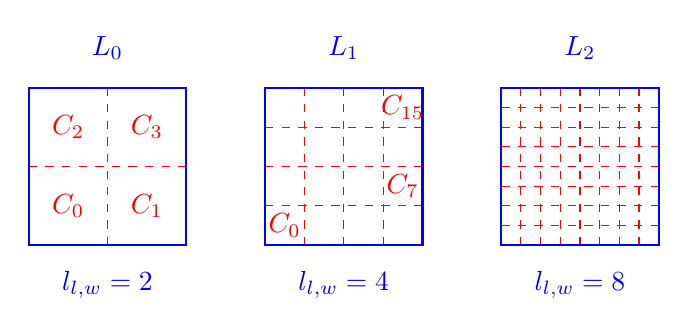
\begin{tikzpicture}
		\foreach \x/\step/\lw in {0/1/2,1/.5/4,2/.25/8} {
			\draw[red, dashed, step=\step] (3 * \x, 0) grid (3 * \x + 2, 2);
			\node[blue] at (1 + \x * 3, -.5) {\(l_{l,w}=\lw\)};
		}
		\draw[blue, thick] (0,0) rectangle (2,2);
		\draw[blue, thick] (3,0) rectangle (5,2);
		\draw[blue, thick] (6,0) rectangle (8,2);
		
		\foreach \l in {0,1,2} {
			\node[blue] at (1 + \l * 3, 2.5) {\(L_{\l}\)};
		}
		
		\node[red] at (.5,.5) {\(C_0\)};
		\node[red] at (1.5,.5) {\(C_1\)};
		\node[red] at (.5,1.5) {\(C_2\)};
		\node[red] at (1.5,1.5) {\(C_3\)};
		
		\node[red] at (3.25,.25) {\(C_0\)};
		\node[red] at (4.75,.75) {\(C_{7}\)};
		\node[red] at (4.75,1.75) {\(C_{15}\)};
		\end{tikzpicture}
	\end{figure}
	\paragraph{Clusters}\label{sec:clusters}
	The clusters group points in an area into small chunks. Figure \ref{fig:points2} shows that their width and height are defined as \(c_{a,w}\) and \(c_{a,h}\). The absolute position \((c_x,c_y)\), meaning the lower left corner, of a cluster can be described as \(c_x(C_i) = l_x + (i \mod l_{l,w}) \times c_{a,w}\) and \(c_y(C_i) = l_y + (i \mod l_{l,h}) \times c_{a,h}\). These two formulas first get the row and column of the cluster and then transform them absolute coordinates. The logical behind it should be trivial.\\	
	Analogous to the levels, clusters have too logical dimensions. \(c_{l,w}\) and \(c_{l,h}\) refer to the amount of points they are wide and high. They are given by settings and equal for all clusters in the entire dataset. As seen in Figure \ref{fig:points2}, clusters index the points they contain as well. This procedure is analogous to the indexing of clusters. The index \(i\) of a point \(P_i\) can be described as \(i = h + k \times c_{l,w}\), where \(h\) is the column and \(k\) is the row of the point do describe. The position \((P_x|P_y)\) of a point \(i\) can be described as \(P_x = c_x + (i \mod c_{l,w}) \times p\) and \(P_y = c_y + \lfloor (i / c_{l,w}) \rfloor \times p\).\\
	\(c_{a,w}\) and \(c_{a,h}\) change with the depth of the cluster they are in. They are defined as the following:
	\[c_{a,w}(C) = \frac{l_{a,w}}{l_{l,w}(L(C))}\]
	The same applies analogous for \(c_{a,h}\)
	The link between \(p(L_d)\) and \(d\) can now be established. The following can be inferred from Figure \ref{fig:dataset}:
	\[p(L_0) = \frac{l_{a,w}}{l_{l,w}(L_0) \times c_{l,w}}\]
	\[p(L_d) = \frac{l_{a,w}}{l_{l,w}(L_d) \times c_{l,w}} = \frac{l_{a,w}}{l_{l,w}(L_0) \times f^d \times c_{l,w}}\]
	\(c_{l,w}\) and \(l_{a,w}\) are the equivalent for each cluster or level and thus do not refer to one. It should be noted that \(p(C) = p(L(C))\), since clusters contain the same points as the level they are in. It can be inferred from \ref{fig:points2} that \(p(C) = \frac{c_{a,w}}{c_{l,w}(C)}\)\\
	\begin{figure}
		\centering
		\caption{Points in a cluster}
		\label{fig:points2}
		\begin{minipage}{.4\textwidth}
			\centering
			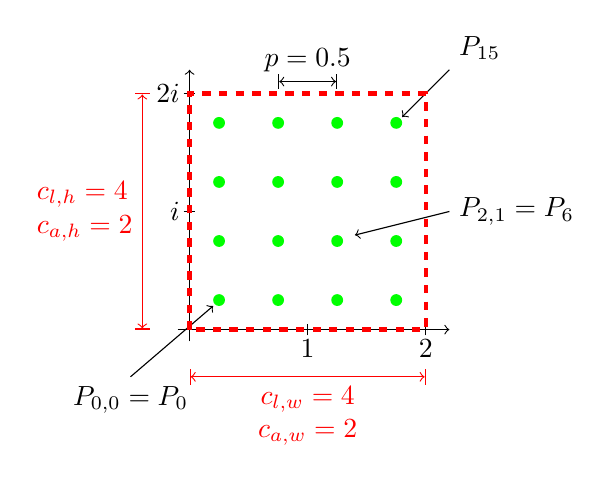
\begin{tikzpicture}[scale=1.5]
			\draw[->] (0,-.1) -- (0,1) node[left] {$i$} -- (0,2) node[left] {$2 i$} -- (0,2.2);
			\draw[->] (-.1,0) -- (1,0) node[below] {$1$} -- (2,0) node[below] {$2$} -- (2.2,0);
			\draw (-.05,1) -- (.05,1);
			\draw (-.05,2) -- (.05,2);
			\draw (1,-.05) -- (1,.05);
			\draw (2,-.05) -- (2,.05);
			
			\foreach \x in {0,1,2,3} {
				\foreach \y in {0,1,2,3}{
					\fill[green] (.5 * \x + .25,.5 * \y + .25) circle[radius=.05];
				}	
			}
			\draw[->] (2.2, 1) node[right] {\(P_{2,1} = P_{6}\)} -- (1.4, 0.8);
			\draw[->] (-.5, -.4) node[below] {\(P_{0,0} = P_{0}\)} -- (.2, .2);
			\draw[|<->|] (.75, 2.1) -- (1, 2.1) node[above] {\(p = 0.5\)} -- (1.25, 2.1);
			
			\draw[->] (2.2, 2.2) node[above right] {\(P_{15}\)}-- (1.8, 1.8);
			
			\draw[|<->|, red] (-.4,0) -- (-.4,1) node[left,align=left] {\(c_{l,h} = 4\)\\\(c_{a,h} = 2\)} -- (-.4, 2);
			\draw[|<->|, red] (0,-.4) -- (1,-.4) node[below,align=center] {\(c_{l,w} = 4\)\\\(c_{a,w} = 2\)} -- (2,-.4);
			
			\draw[red, ultra thick, dashed] (0,0) rectangle (2,2);
			\end{tikzpicture}
		\end{minipage}
	\end{figure}
	
	\subsubsection{Fractal Calculator}
	%TODO does this help?
	\begin{figure}
		\caption{Schematic of the calculator}
		\label{fig:calculator_schematic}
		\centering
		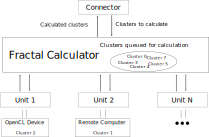
\includegraphics[width=\textwidth]{res/images/calculator.png}
	\end{figure}
	The workload which is done by my program is highly parallelizable: each point can be calculated on its own, without any dependence on other points. Such task are usually not performed on a CPU, since they are specially optimized for fast serial computations and suffer from the inability of only taking little advantage of parallization. The component suited for that is the GPU, which can usually compute hundreds if not thousand of operations simultaneously. It is also possible to distribute the work among multiple devices, should as system have more than one GPU for example.\\
	Java however has no native way of accessing GPUs, and I thus had to fall back onto another programming language, OpenCL. OpenCL (Open Computing Language) is able to address GPUs and use them for computations. The caveat however is that OpenCL works on a C based design, meaning that I as a programmer have to worry much more about coding than I would in Java, where some work is done by the running JVM, especially regarding memory management. It is to note that not every CPU or GPU has proper drivers supporting OpenCL, so my program may not run at all on some system.\\
	Figure \ref{fig:calculator_schematic} shows the calculator from the inside. The connector sends the clusters which need to be calculated to the calculator manager, which distributes them on the calculator units.
	\paragraph{Calculator Units}
	To facilitate the usage of OpenCL devices, each of them is wrapped by a calculator unit. The calculator unit takes care of the manual management required by OpenCL, such as initialization of the device, sending a signal to start the calculation to the device and querying the result back to Java once the calculation has completed.
	\paragraph{Calculator Units Management}
	To start the calculation a list of clusters to create is passed to the calculator. If only one unit exists, which is the common case on computers, it can sequentially get every cluster, compute it and mark it as done. However, things get messier if multiple units exist. Assume that two units try to simultaneously get the next cluster to calculate. This would inevitably lead to a crash or unintended program behavior. To eliminate that risk the calculator has to synchronize access to and from the calculator units.
	\paragraph{Remote Calculator Units}
	If the power of the current machine is not sufficient for the calculations, the work can be split over other machines via Internet. One computer then acts as the ``master'', which organizes the calculation. All other machines are ``slaves'' and connect to the master to offer him their services. From the calculators perspective the slaves are calculator units, and thus sees no difference between a remote machine and for example an installed GPU. The units wrapping remote computers have of course a different implementation than the normal ones. They have to handle the connection and make sure that data is sent and received correctly.\\
	One central thing to consider when using remote connections is the latency. While commands can be sent almost instantly to a GPU it may take many milliseconds to send it to another machine over the Internet, which is a lot on a computer that can perform hundreds of operations in just a picosecond. It is thus crucial to send as little data as possible. This can be achieved by buffering data, which means that the program avoids sending many small datapackets but instead sends few big ones.
	\subsubsection{Image Generator}\label{sec:image_generation}
	The last act to functionality in my program is the visualization of the data, which is done by the image generator. It queries the data needed from the dataset and maps the values to a color. The procedure is divided in multiple smaller steps, which are illustrated in Figure \ref{fig:img_gen}. The yellow grid represents the image, where each cell is a pixel.
	\paragraph{Step One to Four}
	When the program wants to create an image the parameters have to be given, which are the width \(I_{l,w}\) and height \(I_{l,h}\) in pixels and the area to render, whose width and height are given by \(I_{a,w}\) and \(I_{a,h}\). It should be trivial that \(\frac{I_{l,h}}{I_{l,w}} = \frac{I_{a,h}}{I_{a,w}}\). With the help of these the image generator finds out which points of the dataset are needed. Because the pixels are on a raster, the distance \(p(I)\) between two neighboring pixels is always the same, meaning that the datapoints used to create it have too the same distance to the their neighbors. This comes in handy since the dataset sorts the points by the same metric, meaning that the points needed for the image are all in one level \(L(I)\). While it might seem that \(p(I) = p(L(I))\) so that the points can be matched exactly it is suffices that \(p(I) \geq p(L(I))\). The will be harked back later. When the level is known, the clusters needed can be determined. This is done by simply determining which clusters overlap with the area of the image.
	\paragraph{Step five and six}
	The clusters are mapped to an interim image \(R(I)\), which has as inferred from the figure the same amount of pixels as all needed clusters have points. Each point then corresponds to a pixel, which is colored according to the point's value. To determine which value corresponds to which color the program utilizes a color function, which takes a value as an argument and returns the color (in hexdecimal RGB format) associated with it. Note that the function also depends on the maximal amount of iterations the program tried on that point. The color function can be freely manipulated by the user before starting the image creator since it is coded in OpenCL.\\
	The interim image covers as seen in the figure more area than requested. It is thus cropped down. But this alone does not suffice, the image also has to be scaled down to the resolution given by the requested image. This is because the \(p(L(I))\), which was used for \(R(I)\), is equals or smaller than \(p(I)\). This can broadly be interpreted that \(R(I)\) has ``smaller'' pixels than \(R(I)\), thus needing more pixels to fill the same area. The scaled image can then be returned to the caller.\\
	Attentive readers might detect an issue here: the points are moved slightly around to fit the next best pixels location, shifting the image slightly. Although this is a greater issues on this example with such a small image, but this effect becomes negligible on bigger images, since the points are moved at most by one pixel.\\
	A much greater quality issue is the scaling algorithm (called ``nearest neighbor''). Because my work does not focus on that aspect, I have used the most simple one, which while being fast can have drastic quality issues. This can is best seen in videos, where a lot of noise is generated.\\
	\paragraph{Buffering of \(R(I)\)}
	While moving around and zooming around, the user often sees the approximately same area, meaning that for these images the same clusters are going to be rendered. I this thus sensible to store the \(R(I)\) generated in a buffer. If a new image has to be created the image creator checks first if the area has already once been rendered, and if so it can skip step five, which is the most time costly. The drawback is that these stored images will with time slowly use a lot of memory.
	\paragraph{Video creation}
	It is also possible to create a video in my program. A video is nothing more than many images displayed fastly one after another. The program thus just creates many images and connects them to a video. The process of combining images to a video is done by invoking a specialized program called FFMPEG \cite{FFMPEG}, which has to be installed on the system in order to be used. Since the video creation is not particularly interesting I will not go in greater depth than this.
	\begin{figure}
		\centering
		\caption{Image generation course}
		\label{fig:img_gen}
		\begin{minipage}{.4\textwidth}
			\centering
			\caption*{1: Image Parameters}
			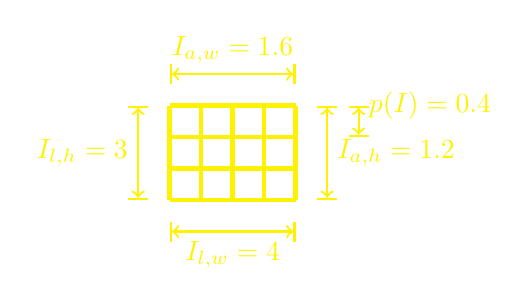
\begin{tikzpicture}
			\draw[ultra thick, yellow,step=.4] (0,0) grid (1.6,1.2);
			\draw[|<->|, yellow, thick] (-.4, 0) -- (-.4, .6) node[left] {\(I_{l,h} = 3\)} -- (-.4, 1.2);
			\draw[|<->|, yellow, thick] (0,-.4) -- (.8,-.4) node[below] {\(I_{l,w} = 4\)} -- (1.6,-.4);
			\draw[|<->|, yellow, thick] (2, 0) -- (2, .6) node[right] {\(I_{a,h} = 1.2\)} -- (2, 1.2);
			\draw[|<->|, yellow, thick] (0,1.6) -- (.8,1.6) node[above] {\(I_{a,w} = 1.6\)} -- (1.6,1.6);
			\draw[|<->|, yellow, thick] (2.4, .8) -- (2.4, 1) -- (2.4, 1.2) node[right] {\(p(I) = 0.4\)};
			\end{tikzpicture}
		\end{minipage}
		\begin{minipage}{.4\textwidth}
			\centering
			\caption*{2: Image location and size, whole dataset for reference}
			\begin{tikzpicture}
			\node at (2,2) {\includegraphics[width=4cm, height=4cm]{res/images/mandelbrot.png}};
			\draw[thick, orange, ->] (-.3,2) -- (4.3,2) node[right]{\(Re\)};
			\draw[thick, orange, ->] (2,-.3) -- (2,4.3) node[right]{\(Im\)};
			\draw[ultra thick] (0,0) rectangle (4,4);
			
			\draw[orange](1.9,3) -- (2.1,3) node[right] {\(i\)};
			\draw[orange](1.9,4) -- (2.1,4) node[right] {\(2i\)};
			\draw[orange](3,1.9) -- (3,2.1) node[above] {\(1\)};
			\draw[orange](4,1.9) -- (4,2.1) node[above] {\(2\)};
			
			\draw[ultra thick, yellow,step=.4] (1.199,1.199) grid (2.8,2.4);
			\end{tikzpicture}
		\end{minipage}
		\begin{minipage}{.4\textwidth}
			\centering
			\caption*{3: Selecting the level}
			\begin{tikzpicture}
			\node at (2,2) {\includegraphics[width=4cm, height=4cm]{res/images/mandelbrot.png}};
			\draw[ultra thick, blue] (0,0) rectangle (4,4);
			\foreach \x in {0,...,15} {
				\foreach \y in {0,...,15}{
					\fill[green] (.25 * \x + .125, .25 * \y + .125) circle[radius=.05];
				}	
			}
			\draw (4.3, .625) -- (4.3, .75);
			\draw[ultra thick, yellow,step=.4] (1.199,1.199) grid (2.8,2.4);
			\end{tikzpicture}
		\end{minipage}
		\begin{minipage}{.4\textwidth}
			\centering
			\caption*{4: Selecting the clusters}
			\begin{tikzpicture}
			\node at (2,2) {\includegraphics[width=4cm, height=4cm]{res/images/mandelbrot.png}};
			\draw[ultra thick, blue] (0,0) rectangle (4,4);
			\draw[step=1,red, dashed] (.99,.99) grid (3,3);
			\foreach \x in {4,...,11} {
				\foreach \y in {4,...,11}{
					\fill[green] (.25 * \x + .125, .25 * \y + .125) circle[radius=.05];
				}
			}
			\draw[ultra thick, yellow,step=.4] (1.199,1.199) grid (2.8,2.4);
			\end{tikzpicture}
		\end{minipage}
		\begin{minipage}{.4\textwidth}
			\centering
			\caption*{5: Creating an image from the clusters}
			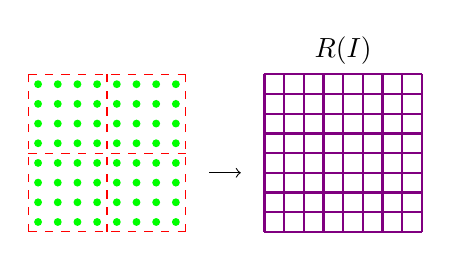
\begin{tikzpicture}
			\draw[step=1,red, dashed] (0,0) grid (2,2);
			\foreach \x in {0,...,7} {
				\foreach \y in {0,...,7}{
					\fill[green] (.25 * \x + .125, .25 * \y + .125) circle[radius=.05];
				}
			}
			\draw[->] (2.3, .75) -- (2.7, .75);
			\draw[step=.25, violet, thick] (2.99,0) grid (5,2);
			\node[above] at (4, 2) {\(R(I)\)};
			\end{tikzpicture}
		\end{minipage}
		\begin{minipage}{.4\textwidth}
			\centering
			\caption*{6: Cropping and scaling the interim result}
			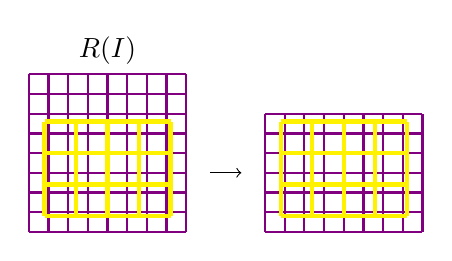
\begin{tikzpicture}
			\draw[step=.25, violet, thick] (0,0) grid (2,2);
			\node[above] at (1, 2) {\(R(I)\)};
			\draw[ultra thick, yellow,step=.4,shift={(.2,.2)}] (0,0) grid (1.6,1.2);
			\draw[->] (2.3, .75) -- (2.7, .75);
			
			\draw[step=.25, violet, thick,shift={(3,0)}] (0,0) grid (2,1.5);
			\draw[ultra thick, yellow,step=.4,shift={(3.2,.2)}] (0,0) grid (1.6,1.2);
			\end{tikzpicture}
		\end{minipage}
	\end{figure}
	\subsection{Data Calculation and Image Generation Course}
	This section will shorty cover the programs executions course, tying the previously discussed sections together. When the program starts, the dataset is initialized. The parameters passed to it during its creation are the location of the dataset, \(f\), \(l_{a,a}\), \(l_{a,h}\), \(l_{l,w}(L_0)\), \(l_{l,h}(L_0)\), \(c_{l,w}\) and \(c_{l,h}\). The initial parameters are defined in the settings and can be changed there. They are used to deduce the parameters of any other level, cluster or point.\\
	When a new image is needed, the connector asks the dataset for the clusters needed. If any of these clusters have not yet been calculated the connector sends them to the fractal calculator to create them. Next, the image creator checks if the clusters has already been rendered once as an interim result, and renders the clusters if not. The interim result is then cropped and resized, and then finally sent back to the GUI which has requested the image.
	\section{Reflection}
	I would like to use this last section of my work to add my personal thoughts to my senior paper and to neatly close the discussion around my work.
	\subsection{Limitations, Bugs and Workarounds}
	Programs naturally come with hidden bugs and limitations. As my program became bigger more bugs to be squashed arose. I have due to time issues not been able to tackle every one and thus am obliged to shortly describe the bugs. One bug is also induced by factors outside of my range such as driver support.
	\paragraph{OpenCL on Macs}
	Apple decided to stop supporting OpenCL on its devices \cite{appleinsider}. Although the program detects the GPU and CPU as OpenCL devices, only the latter works.
	\paragraph{Magnification Limit}
	Every cluster \(C_i\) has an index \(i\) to store their location. This index is stored in a Java \verb|int| which can usually only assume values up to \(2^{64} - 1\). If the program tries to allocate a cluster with a higher index the program crashes due to a numerical overflow. This happens when \(l_{l,w} \times l_{l,h}\) is greater than the aforementioned value because \(i = a + b \times l_{l,w}\) where \(0 \leq a < l_{l,w}\) and \(0 \leq b < l_{l,h}\).\\
	If due to this it is no possible to render a specific area the following workaround is recommended: restart the application, but set the levels' position and dimension to the previously unavailable area.
	\paragraph{Memory Constraints}\label{sec:memory_problem}
	As the program calculates new values it stores them in RAM and VRAM, which both are limited in size. Without freeing any RAM during runtime the program is bound to try to allocate more RAM when no more is available, leading to a crash caused by an \verb|OutOfMemoryError|.
	\paragraph{Floating-Point precision}
	Floating point math on computers is if no special workarounds are used always tied to the machine precision, meaning that small rounding error occur during calculations. While the error is negligible on normally used numbers it can have devastating effects when the numbers become too small to be represented correctly. In my program this happens when the precision \(p\) becomes smaller than \(10^{-13}\), causing the values to be miscalculated.
	\subsection{Workflow}
	Programming an application of this size has come with many unexpected challenges which are tied to the nature of computer science. These challenges have, when not accounted for, caused either several delays in my time schedule or forced me to not implement a feature.
	\paragraph{Structure Design}
	The design as it is present now was the result of a long journey. At the very beginning it consisted of a simple program that calculated points of the Mandelbrot set, wrote the result into a file and then quit. It was all in just one file, without any logical structure. Because of the small size changes were easily introduced. However, new functionalities naturally increased the programs complexity by many times. The code was grouped in multiple modules which each took over a function. The advantage of modules is the ability to make internal changes to one without affecting other modules. This however does not hold true for any changes to the overall model, since this affects all modules. This happened quite often as I made many model changes due to me having taken either shortsighted decisions or simply making a faulty designs, costing me much time. The most extreme cases were the redesign of the database and the introduction of OpenCL.\\
	The first database created was similarly to the current cluster based, but had serious design flaws related to memory usage as it would reserve lots of RAM for data that was not guaranteed to be calculated. Because all other crucial components depend on the database's implementation, they were all forced follow the changes made there.\\
	Since I had never programmed in OpenCL before I had no knowledge what kind of structure would suit the addition of OpenCL supported calculations. Upon its introduction to my code is was still only halfway aware of how worked, making the design choices based solely by best guesses. Since OpenCL does not use the same RAM the program the additional challenge arose manually manage, i.e. allocate and free, RAM in a C like style, which is ironic since one of the reasons I coded in Java is to not have to worry about memory allocations and deallocations.\\
	Another time stealing mistake of mine was the opposite making a design not future proof. Thinking too big I made parts of the model more complex than they ultimately needed to be. An example is the way a points value is represented. Whereas it is just a simple \verb|int| in the final version it used to be more class, which made it more cumbersome to perform operations on it and also resulted in a slight performance penalty.
	\paragraph{Squashing bugs}
	One of the most banal and trivial hardships encountered are logical errors in the code, causing either simple misbehavior or runtime crashes. These can be prevented by using assertions. They are checks done at runtime to detect any illegal or senseless program states. If the check fails an \verb|AssertionError| is thrown to let the programmer know that there are issues in his code. I have used these extensively in combination with the OpenCL API.\\
	Assertions alone however are not enough. Sometimes it is useful to pause the execution and inspect the program state manually. This can be done by attaching a debugger to the running program. The debugger is able to pause the program execution at any moment and lets the programmer see the current state. It is also possible to set breakpoints, which cause the debugger to automatically pause execution when such a point is reached. Furthermore, it also pauses when an exception is about to be thrown. This was the most practical use for me since I was able to examine the cause leading to the exception.\\
	The Java debugger however has its limits: It does not work on OpenCL code. This was quite inconvenient because the entire JVM crashes without any useful information if faulty parameters are passed to OpenCL functions, making the search for bugs quite cumbersome.
	\subsection{Possible enhancements}\label{sec:poss_enh}
	The following sections shortly describe what features I would have added to my program if I have had any more time. Neither of them are crucial for my program but each of them would nonetheless bring more stability or comfort.
	\paragraph{OpenGL}
	Although the Java Swing Toolkit which is responsible for the GUI has longtime been replaced by newer alternatives I have decided to use it because it is the only type of GUI of which I am able to program. As of now, the image data has to be passed from OpenCL to the Java Swing application, resulting in a high latency and waste of resources. Had I had more time I would have made effort to implement an OpenGL GUI, which has features to work directly with OpenCL, saving valuable computing power. Another caveat is that since OpenCL works with native machine code it is more responsive and faster than the in any Java code.
	\paragraph{Memory to Disk}
	As mentioned in section \ref{sec:memory_problem}, the memory is a main cause of trouble when the application runs for long a duration. A possibility to combat this problem could be to offload unused data onto the disk, which as - in comparison to RAM - more than enough free space. The caveat here is to determine which data will probably not be used in the near future.
	\paragraph{Dynamic Iterations}
	A question left unanswered in my senior paper is the amount of iterations a point should go before it is considered part of the Mandelbrot set. The general rule of thumb is that the smaller the clip of the fractal is i.e. the closer the points to calculate are the more iterations are necessary to see a clear picture. In my program however the amount of iterations per point is indifferent to the distance between the points \(d\). Dynamically changing the maximal amount of iterations would drastically speed up the calculation of clips with a lower resolution and increase the quality of clips which have zoomed in greatly.\\
	This feature is already for the most part implemented in the program making it possible to give levels which are deeper more iterations. However I have not made any efforts to improve this feature because I simply lacked the time to investigate about how to determine the appropriate amount of iterations for a point.\\
	The default iteration model is named ``static'' and uses the same amount of iterations for every level. A not thoroughly tested variant named ``antiProportional'' can be selected in the settings, which increases the amount of iterations anti proportionally.
	\subsection{Conclusion}
	As described section \ref{sec:poss_enh} I was not able to implement every aspect I wanted to be included. However I can proudly present a program that meets all basic requirements I have given, such as being able to harness the power of a graphics card or exporting videos. Looking back at my work I can say that I made the mistake of investing too much time in the program and by far not enough in the paper. I had not thought that writing down my ideas in an understandable way was going to take way less time. Lastly I would like to thank Mr. Holzer for giving advice, guiding and supporting me through my first greater piece of work.
	\printbibliography
	
	\newcommand{\glossaryentry}[2]{\textbf{#1}&#2\\} %add to the top of the document
	\appendix
	\section{User Guide for the Program}
	\section{Glossary} % add this to where you want your glossary to be
	\noindent
	\begin{tabular}{@{}p{4cm}@{\hspace{12pt}}p{0.75\textwidth}@{}}
		\glossaryentry{term}{asldjfdsalkf lslökaslköflsadk jlksadj lsa djlsa jdkösaljk lsdkjf lasfj asdj fdsa jfo ijsd ffdsalöjsadj ldsa jflsdajöl jdsl lsa d}
		\glossaryentry{term}{asldjfdsalkf lslökaslköflsadk jlksadj lsa djlsa jdkösaljk lsdkjf lasfj asdj fdsa jfo ijsd ffdsalöjsadj ldsa jflsdajöl jdsl lsa d}
		\glossaryentry{term}{asldjfdsalkf lslökaslköflsadk jlksadj lsa djlsa jdkösaljk lsdkjf lasfj asdj fdsa jfo ijsd ffdsalöjsadj ldsa jflsdajöl jdsl lsa d}
		\glossaryentry{term}{asldjfdsalkf lslökaslköflsadk jlksadj lsa djlsa jdkösaljk lsdkjf lasfj asdj fdsa jfo ijsd ffdsalöjsadj ldsa jflsdajöl jdsl lsa d}
		\glossaryentry{term}{asldjfdsalkf lslökaslköflsadk jlksadj lsa djlsa jdkösaljk lsdkjf lasfj asdj fdsa jfo ijsd ffdsalöjsadj ldsa jflsdajöl jdsl lsa d}
		\glossaryentry{term}{asldjfdsalkf lslökaslköflsadk jlksadj lsa djlsa jdkösaljk lsdkjf lasfj asdj fdsa jfo ijsd ffdsalöjsadj ldsa jflsdajöl jdsl lsa d}
	\end{tabular}
\end{document}